\section{Design} \label{design}

When analysing the problem, it was clear there were 3 distinct parts:
\begin{itemize}
    \item Parsing user input.
    \item Evaluating the expression.
    \item Visualising the expression.
\end{itemize}
By implementing each part individually and then tying them together with a well defined interface, each part could be individually tested, and changes to one would not affect the others.

\subsection{Language}
The first design decision to make was which language to implement the visualiser in. Most languages are perfectly suitable for the job, with extensive libraries and tooling, but picking the one for the task early would allow me to research existing solutions to the further sections.

An obvious choice would be to use Haskell, with a variety of existing tools for parsing Haskell within itself, such as ghc-vis for visualising data structures. However, despite making a visualiser for it, my knowledge with it's built-in library and syntax was not great. I was going to learn a lot about Haskell while making the visualiser, but I would encounter many hurdles if I was to use it. While the user of such a visualiser would likely already have Haskell installed, a beginner would need to install the project.

My next choice was JavaScript, a language that I am much more familiar with. It has a much larger range of libraries and online information. JavaScript also has the advantage of being the primary language on the web, allowing extremely easy access by going to a site hosting the visualiser.
To reduce complexity, I decided to keep it as a static site, with all the logic on the client-side. This meant I didn't have to produce a server and handle communication between it and the client.

\subsection{Lexing and Parsing}
Within JavaScript, a variety of community made parsers exist \cite{antlr4,ohmjs} that can take a specific grammar and generate a parser. However, these tools parse into a representation that would need to be further converted into an implementation that could work with the other sections of the project.

Therefore I decided I would make my own parser. The main requirements was an easy to implement, and extensible parser so features of Haskell could be implemented incrementally. The visualiser would primarily be used for small code snippets, so while efficiency was important, it was not the most crucial aspect.

To satisfy these requirements, I investigated various types of parsers. The most common distinctions being LL(k) and LR(k) parsers, or top-down and bottom-up, where "k" are the number of lookahead tokens. LL parsers are typically easy to manually create, but are much harder to run in linear time as they may have to backtrack when reaching dead-ends while parsing. LR parsers are the opposite, typically requiring specialised tools to create the tables necessary to parse within linear time with no backtracking or guesswork.\cite{Syme2007}.

The choice was clear, an LL parser would fit perfectly. Care would have to be taken to keep the time complexity down, but the ease of use and extensibility would more than make up for it.

While plain text can be parsed into Haskell directly, it is much easier to pre-process the data with a lexer, converting the input stream into a stream of tokens. This removes extraneous characters, such as insignificant whitespace, and groups characters into labelled tokens. The set of possible tokens is much easier to match on than the set of characters, as the tokens mark the start and end of each construct. This means the lexer's purpose is to divide up the input, and the parser's purpose is only to validate it, separating the problem into two easier problems.

\begin{figure}
\centering
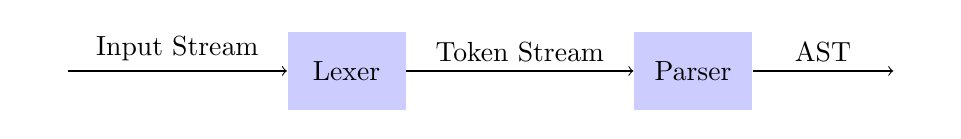
\begin{tikzpicture}[scale=2,
invisible/.style={rectangle, minimum size=5mm},
node/.style={rectangle, fill=blue!20, minimum size=15mm, minimum height=10mm}
]
\node[invisible] (westedge) at (0, 0) {};
\node[node] (lexer) at (1.9, 0) {Lexer};
\node[node] (parser) at (4.1, 0) {Parser};
\node[invisible] (eastedge) at (5.5, 0) {};

\draw[->] (westedge) -- (lexer) node[midway, above] {Input Stream};
\draw[->] (lexer) -- (parser) node[midway, above] {Token Stream};
\draw[->] (parser) -- (eastedge) node[midway, above] {AST};
\end{tikzpicture}

\caption{The flow of data within a parser.}
\label{fig:lexerparserdiagram}
    
\end{figure}

\subsection{The Internal Representation}
As the users input would require additional functionality than just executing, it had to be converted into an internal representation that could be analysed, stepped through, and visualised. Compilation was off the table, as that would lose important information associated with visualising, such as identifier names, and would be very difficult to step through and visualise. Type information can also be discard after successful compilation, as values of one type are never passed into a function that cannot take them, and non-exhaustive pattern matching is generally avoided.\footnote{Unless unsafe functions are used, but they come with many other risks.}

Other interpreted languages, such as Python, Java, and C\#, are compiled into a bytecode and then interpreted via a virtual machine. Bytecodes are a compact and efficient way to store and run an interpreted program, as extraneous characters, such as whitespace, can be stripped, and identifiers simplified. However, in my case, converting the users input into bytecode would lose too much information like compiling, as type information can be removed and identifiers simplified. As the goal is to visualise expressions similarly to the user's input, preserving identifier names is a necessary requirement to ease understanding.

The easiest approach I could think of was an object-oriented style to represent types and thunks. This would allow some aspects of each system to be implemented and tested together, before adding more features later, allowing them to built on top of a strong foundation. By defining an interface for types and an interface for thunks, e.g a method to apply a beta reduction  given the symbol and replacement, a thunk can have any type, any child thunk, e.t.c and handle its case without needing to know about its parent's, or children's information. Another benefit of constructing the types and thunks in a tree structure is that the child thunks and types are still fully formed expressions. This would allow for the user to analyse parts of expressions without errors occurring.

\subsection{Visualising}
As described in Section \ref{visualisationsection}, two classes of visualisers identified were text-based, and graph-based visualisers, each with distinct advantages and disadvantages.

Graph-based visualisers are more visual, and can smoothly transition between states. This allows the user to easily see the changes from one state to another, as they can focus on that part. A number of libraries also exist for visualising graphs, such as \cite{cytoscape}, that are capable of rendering a manipulable graph within a website. In many ways, an abstract syntax tree is already a graph, and, for this project, each thunk could be converted into a node in the diagram, with edges connecting to its children. However, although easier to display as a graph, this style of visualisation not necessarily easier for the user to interpret, as the graph is visually very different from the program the user inputs.

Text-based visualisers aren't as easy to create smooth transitions with, but keep the states very readable. For example, when a term is substituted into an expression, the user will be able to see what the new expression looks like without having to decode a graph, and the user can more easily understand what has happened without understanding exactly how functional programming works. However, few libraries exist, so a way to visualise the expression would have to be implemented manually.

Despite the extra work, I decided to implement the visualiser with a text-based approach, similarly to \cite{visualize-cbn}. This is for the aforementioned reasons, as ease of use was one of the main design goals for the visualiser.